In order to study the motion of the particles a liquid containing particles i pumped through a microfluidic channel. The channel is placed on a moveable stage on top of a microscope so that the particle can be tracked by moving the stage and thus the channel in order to keep the particle stationary above the microscope. A sketch of this setup can be seen in figure \ref{fig:channelsketch} and a photograph of the actual setup in figure \ref{fig:setuppicture}. 


\begin{figure}[H]
\centering
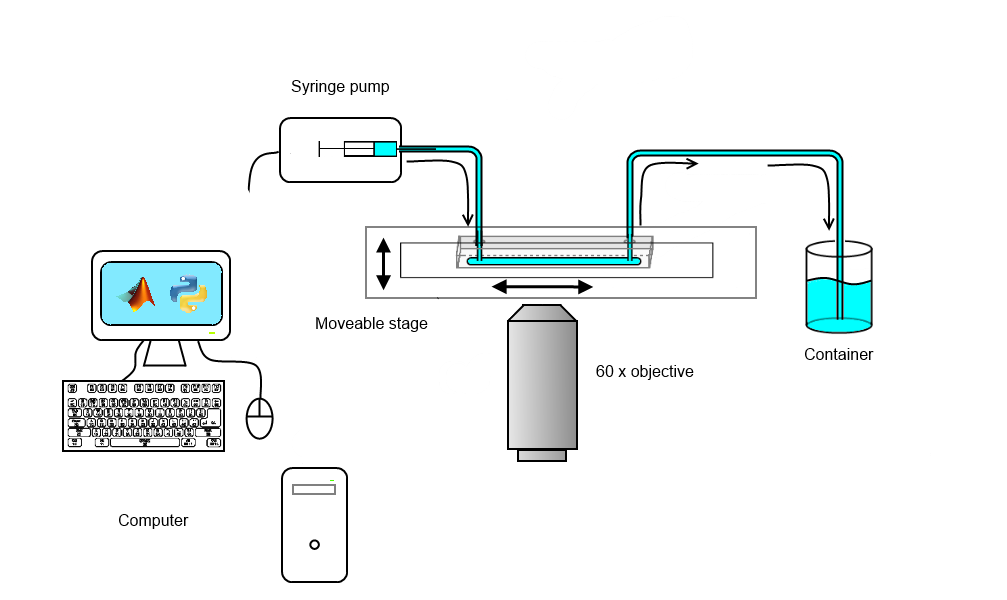
\includegraphics[width=0.8\textwidth]{figures/method/setupsketch.png}
\caption{Sketch of the set up}\label{fig:setupsketch}
\end{figure}

\begin{figure}[H]
\centering
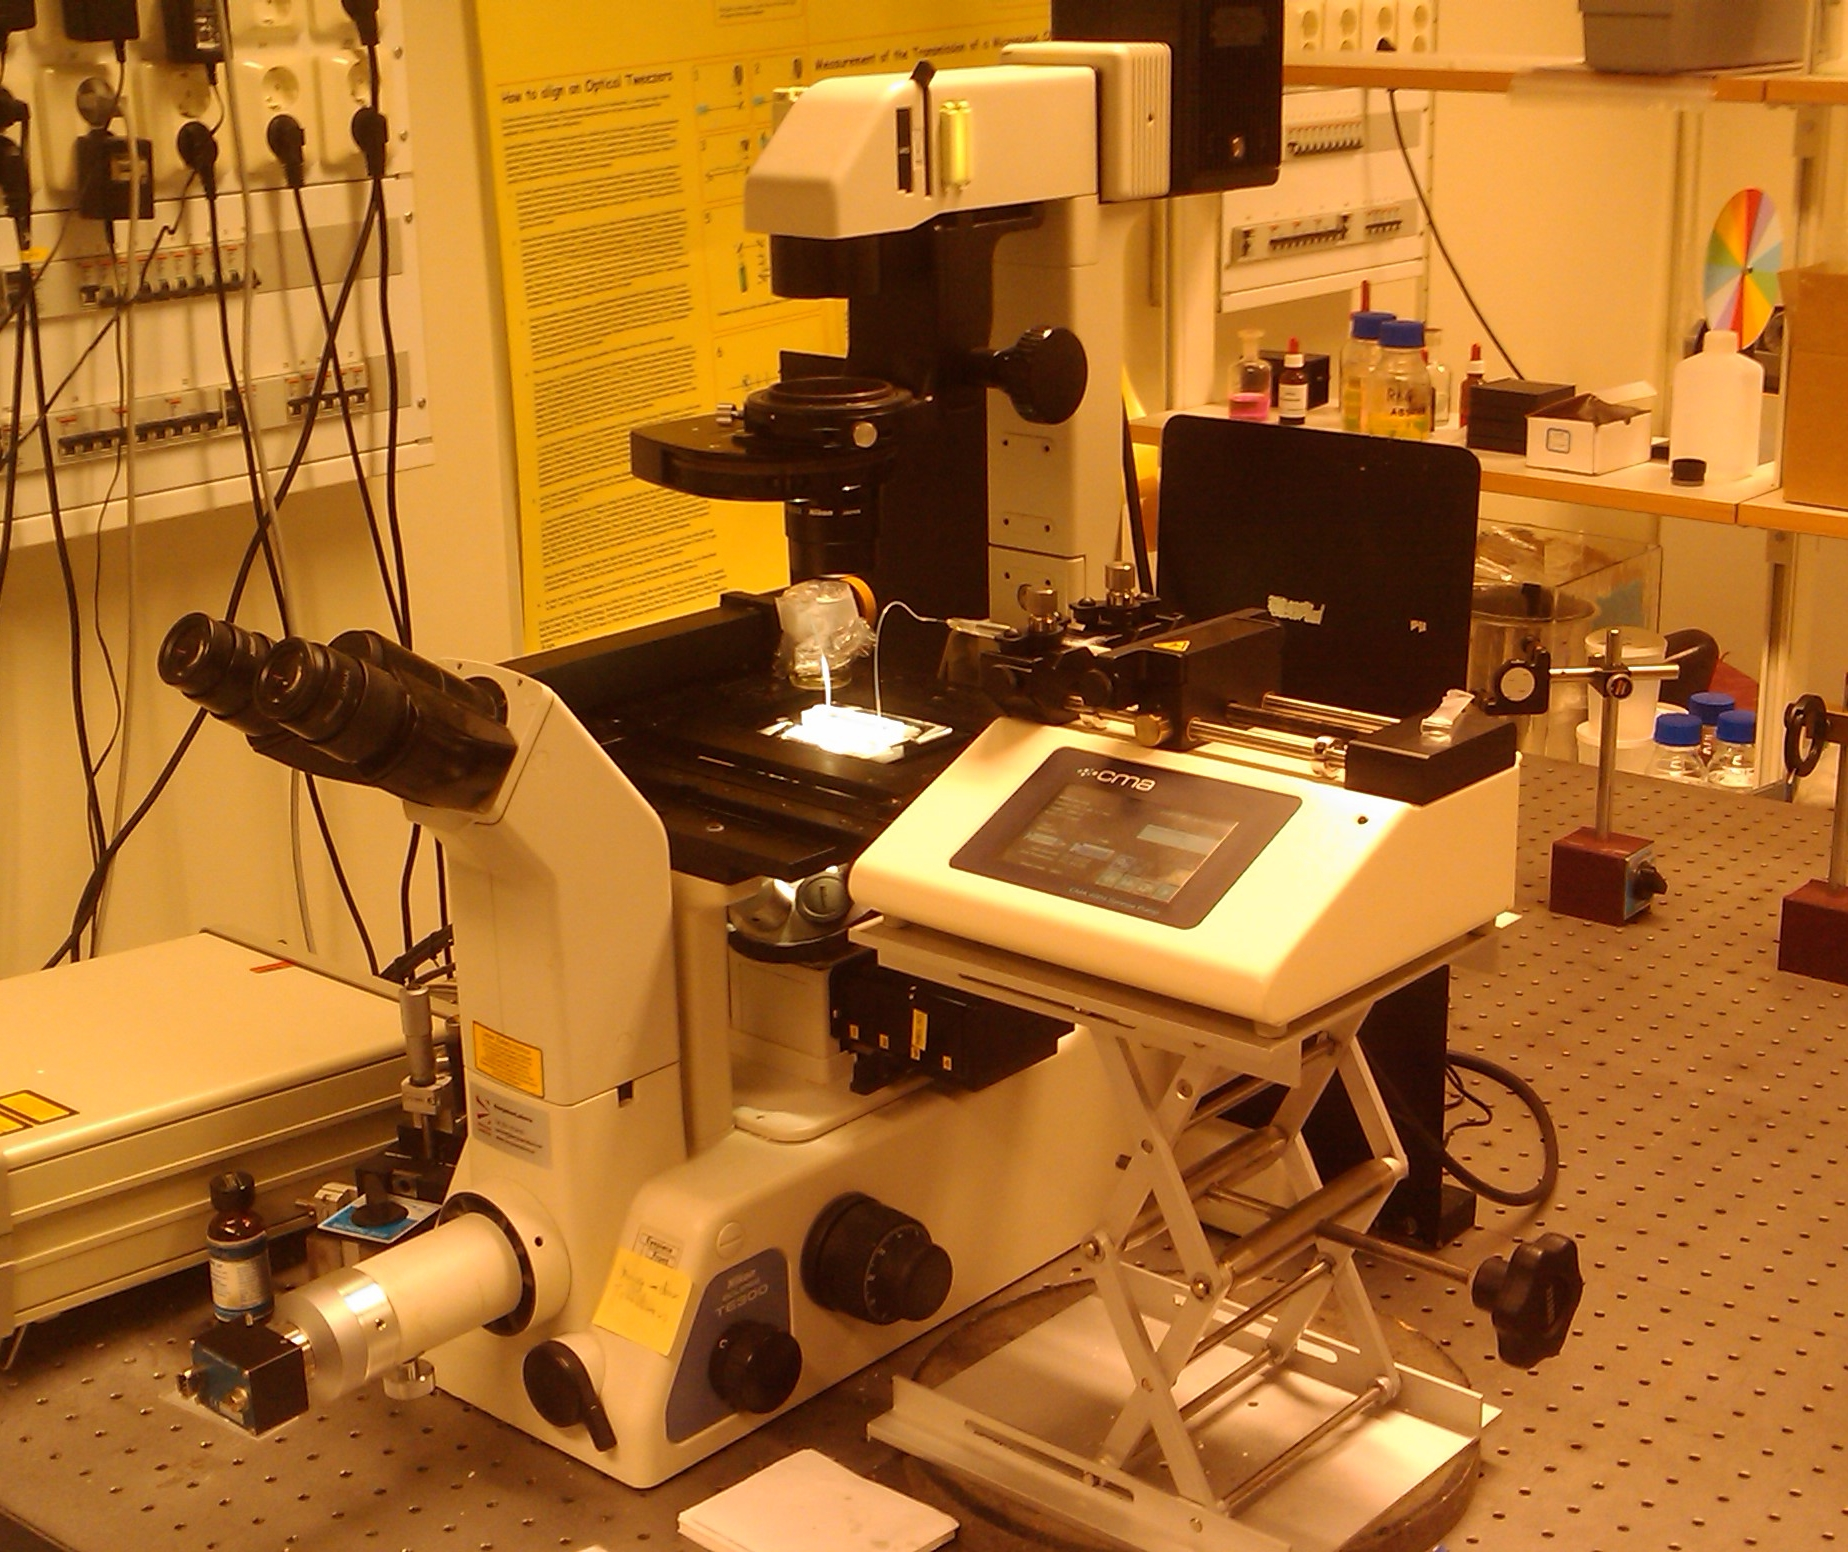
\includegraphics[width=0.8\textwidth]{figures/method/ExperimentalOverview.jpg}
\caption{Overview of the set up}\label{fig:setuppicture}
\end{figure}


The microfluidic channel is \unit[40]{mm} long, \unit[2.5]{mm} wide and ca unit[150]{$\mu$m} deep. The channel is made from Polydimethylsiloxane (PDMS) and plasma bonded to a microscope slide, a more detailed description of the process can be found from the Caroline Workshop \cite{PDMS}. This material and procedure is chosen so that a particle that gets filled with dirt or breaks can cheaply and easily be replaced and because it's non reactive and highly transparent. A sketch of the channel can be seen in figure \ref{fig:channelsketch} and a photograph of an actual channel can be seen in figure \ref{fig:channelpicture}. 

\begin{figure}[H]
\centering
\begin{subfigure}[b]{0.45\textwidth}
\includegraphics[width=0.9\textwidth]{figures/method/channelDetail.pdf}
\caption{Sketch of the channel}\label{fig:channelsketch}
\end{subfigure}
\begin{subfigure}[b]{0.45\textwidth}
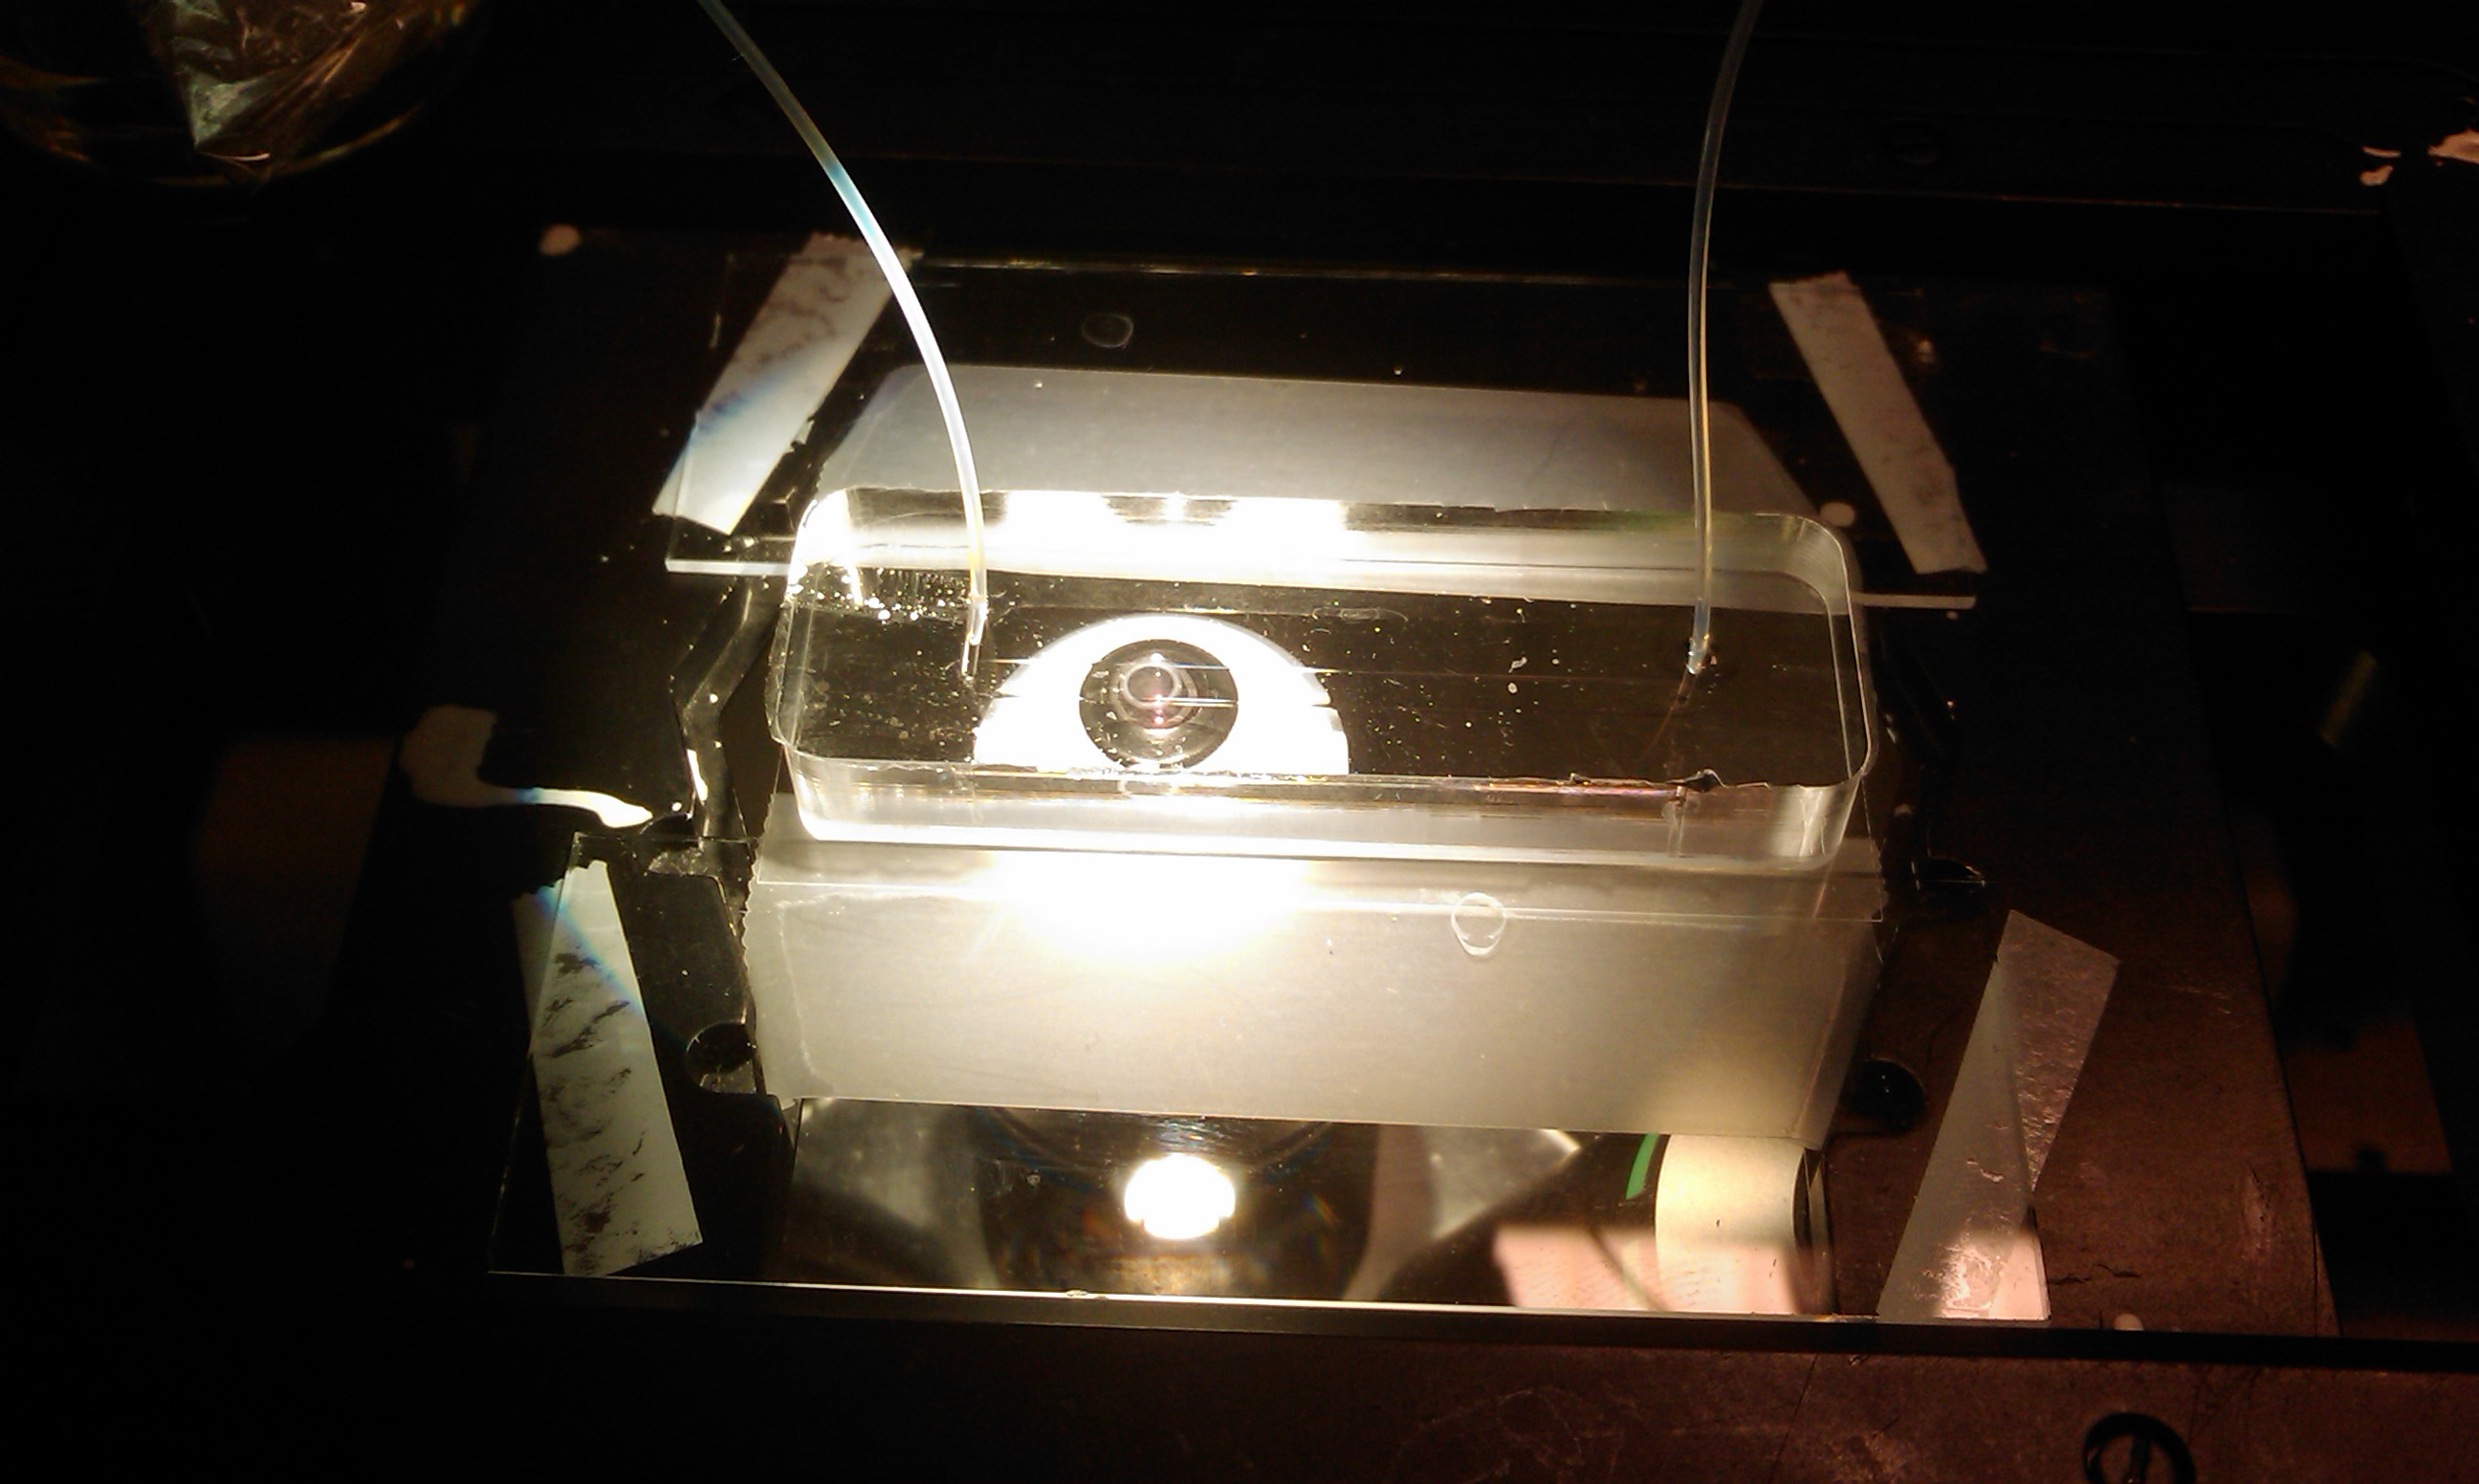
\includegraphics[width=0.9\textwidth]{figures/method/ChannelZoomed.jpg}
\caption{Picture of the channel}\label{fig:channelpicture}
\end{subfigure}
\caption{}
\label{fig:channel}
\end{figure}


To find the maximum flow speed of the channel we need to know the flow profile and using the software used in Johansson \cite{AntonThesis} we get the flow profile that can be seen in figure \ref{fig:flowprofile}. Integrating the flow profile over the entire surface will give us an effective flow area. To find the maximum flow speed we can simply divide the flow rate by the effective flow radius.

DO THIS SOME TIME SOON OKAY?





%Thus two sets of glass particles from Nippon Glass, Japan\cite{Particles}, have been used. 
%They are cylindrical with a consistent width of \unit[3]{$\mu$m} and \unit[5]{$\mu$m} and varying length. Images taken 
%with a STEM microscope can be seen in figure \ref{fig:particlepictures}. 


%While these particles seemingly satisfy the symmetry conditions they are made glass with a density of approximately 
%\unit[2.57]{g/cm$^3$} at \unit[20]{C$^\circ$} which is significantly higher than that of water with a density of 
%\unit[1]{g/cm$^3$} at \unit[20]{C$^\circ$} and glycerol with a density of \unit[1.5]{g/cm$^3$}. Thus to correct for the 
%density and limit sinking or floating the water soluble Sodium metatungstate which at \unit[20]{C$^\circ$} has maximum 
%density of \unit[2.94]{g/cm$^3$}. To increase the viscosity of the liquid around 8\% glycerol is added, resulting in a 
%measured dynamic viscosity of \unit[$24\cdot 10^{-3}$]{Pa s}



% PIcture of the channel meassurements here 




% Picture of channel flow profile
\begin{figure}[H]
\begin{center}
\includegraphics[width=0.7\textwidth]{figures/method/flowprofile.pdf}
\end{center}
\caption{The theoretical estimation of the flow profile. Image used with permission from Johansson \cite{AntonThesis}}
\label{fig:flowprofile}
\end{figure}


To confirm that the flow is a creeping flow we can calculate the maximum Reynolds number using eq \ref{eq:reynolds} and 
our maximum flow speed. The ma

\begin{equation}
\operatorname{Re} = \frac{U L \rho}{\mu} 
\leq \frac{6.66\cdot 10^{-3} \cdot 2.5 \cdot 10^{-3} 2.5 }{24 \cdot 10^{-3}} 
\approx	 	1.6  \cdot 10^{-3} \ll 1
\end{equation}

This should satisfy the conditions of the Jeffrey equations. To track the particles the channel is put in a moveable stage on a confocal microscope. The entire setup can be seen in figure 



\subsection{List of equipment}
 The equipment used during the experiment is as follows
\begin{itemize}
\item Leica DFC350 FX digital camera 
\item Nikon Eclipse TE 300 microscope
\item Nikon 60x water immersion objective
\item Märzhäuser Wetzlar 'LStep-eco' step engine
\item CMA 4004 syringe pump
\end{itemize}

%
%\subsection{Density matching}
%\begin{equation}
%\rho_{a} = 	\frac {m_{a}}{V_{a}} =
%				\frac{V_{b}\rho_{b} + V_{mix}\rho_{mix}}{V_b + V_{mix}} 
%\end{equation}
%So if we want to find $V_{mix}$ we get
%\begin{equation}
%V_{mix} = \frac{ V_{b}(\rho_{b} - \rho_{a})}{\rho_{a} - \rho_{mix}} 
%\end{equation}
%
